\normalfalse \difficiletrue \tdifficilefalse
\correctionfalse

%\UPSTIidClasse{11} % 11 sup, 12 spé
%\newcommand{\UPSTIidClasse}{12}

\exer{Banc Balafre$\star$ \label{C2:09:50}}

\setcounter{question}{0}\UPSTIcompetence[2]{C2-09}
\index{Compétence C2-09}
\index{TEC}
\index{Théorème de l'énergie cinétique}
\index{Banc Balafre}
\ifcorrection
\else
\marginnote{\textbf{Pas de corrigé pour cet exercice.}}
\fi

\ifprof
\else


\begin{obj}
L'objectif est de valider les exigences suivantes.
\begin{itemize}
\item 2.01 -- Couple résistant : le couple résistant exercé par le film d’eau sur le joint (rotor) à \SI{7 000}{tr.min^{-1}} est estimé à$C_{\text{res}} = \SI{100}{N}{m}$. 
\item 2.02 -- loi de commande La vitesse cible maximale $N^{\text{max}}_C = \SI{7 000}{tr.min^{-1}}$ doit être atteinte en moins de $T_{\text{acc}} = \SI{5}{s}$.
\item 2.03 -- Risque de décrochage : le couple maximal demandé au moteur en fonctionnement doit
rester inférieur à $C^{\text{max}}_u /s = \SI{570}{Nm}$ où $C^{\text{max}}_u = \SI{740}{Nm}$ et
$s = 1,3$ est un coefficient de sécurité.
\end{itemize}

Sans cette partie, nous allons vérifier que le moteur modélisé dans la partie
précédente permet de répondre à l’exigence 2.02 concernant la loi de commande. Nous
allons également mettre en évidence la nécessité de réaliser un asservissement de la vitesse
du moteur.
\end{obj}

Données et hypothèses :
\begin{itemize}
\item pendant toute la phase de mise en rotation de la ligne d’arbre, on considérera pour
simplifier l’étude, que le couple résistant sur le joint(rotor) est constant et égal à
$C_{\text{res}}$;
\item le moteur étant commandé à $U_S/f$ constant, on considérera que le couple moteur
(noté $C_m$) est constant pendant la phase d’accélération;
\item le rendement de la liaison pivot réalisée par le palier hydrostatique (double butée)
est $\eta_b = 0,95$ ;
\item le rendement de la liaison pivot réalisée par les roulements à billes est $\eta_b = 0,9$ ;
\item le moment d’inertie du rotor moteur est $J_{\text{mot}} = \SI{1,15}{kgm^2}$ ;
\item le moment d’inertie de l’accouplement à l’arbre moteur est négligé ;
\item plusieurs solutions technologiques (différentes formes internes et différents matériaux)
seront testées pour la nouvelle géométrie de joint. Le moment d’inertie
maximal du joint (rotor) selon l’axe de rotation est $J_{\text{joint}}= \SI{0,92}{kg. m^2}$ ;
\item le moment d’inertie de l’ensemble bda=\{ butée double + arbre + fusible mécanique\} selon l’axe de rotation est $J_{bda} = \SI{0,092}{kg.m^2}$.
\end{itemize}

On considère l’ensemble de la ligne d’arbre (voir figure \autoref{fig_50_01})  $\Sigma=\{ \text{arbre moteur + accouplement
+ fusible mécanique + tube flexible + butée double + Joint (rotor)} \}$.
On notera $\Omega$ la vitesse de rotation $\Omega\left(\Sigma/0\right)$ de la ligne d’arbre par rapport au bâti 0, et
$J_{\Sigma}$  le moment d’inertie de $\Sigma$ par rapport à l’axe de rotation du moteur.

 
\begin{figure}[H]
\centering
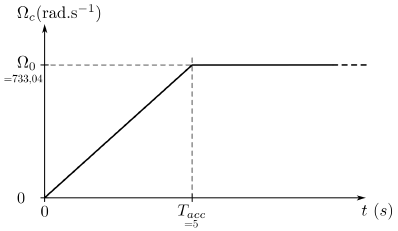
\includegraphics[width=\linewidth]{fig_50_01}
\caption{Représentation en coupe du banc BALAFRE \label{fig_50_01}}
\end{figure}


\fi
 
\question{Exprimer le moment d’inertie $J_{\Sigma}$ en fonction des données fournies et calculer sa valeur numérique.}
\ifprof
\else
\fi

\question{Exprimer l’énergie cinétique de l’ensemble $\Sigma$ par rapport au bâti (noté 0) du banc (fixé au sol).}
\ifprof
\else
\fi

\question{Exprimer la puissance des actions mécaniques extérieures sur $\Sigma$ dans le mouvement de $\Sigma$ par rapport à 0.}
\ifprof
\else
\fi

\question{Exprimer la puissance perdue $P_{\text{pertes}}$ dans les roulements à billes et dans la butée hydrostatique.}
\ifprof
\else
\fi

\question{Exprimer le théorème de l’énergie cinétique appliqué au mouvement de $\Sigma$ par rapport à 0. En déduire l’expression de $\dfrac{\dd \Omega}{\dd t}$ en fonction de $C_m$, $C_{\text{res}}$, $\eta_r$, $\eta_r$ et $J_{\Sigma}$.}
\ifprof
\else
\fi

\question{En explicitant clairement les hypothèses utilisées, expliquer pourquoi
l’accélération peut être considérée constante pendant la mise en mouvement de la ligne
d’arbre.}
\ifprof
\else
\fi

\question{Déterminer la valeur minimale d’accélération $\alpha_{\text{min}}$ compatible avec le
tableau des exigences 2.}
\ifprof
\else
\fi

\question{En déduire la valeur de couple moteur nécessaire pendant cette phase
d’accélération.}
\ifprof
\else
\fi

\ifprof
\else
En cas de perturbation de vitesse sur la ligne d’arbre pendant la phase d’accélération, il
peut se produire un phénomène instable au niveau du film liquide à l’intérieur du joint
testé. Ceci peut se traduire par une perturbation de couple pouvant aller jusqu’à une
valeur $C_p = \SI{100}{Nm}$.
\fi

\question{Déterminer alors la valeur de $C_m$ pour le scénario le plus défavorable.}
\ifprof
\else
\fi

%\question{Conclure vis-à-vis de l’exigence concernant le risque de décrochage du
%moteur. Proposer deux solutions pour éviter le décrochage.}
%\ifprof
%\else
%\fi






\ifprof
\else
\begin{flushright}
\footnotesize{Corrigé  voir \ref{C2:09:50}.}
\end{flushright}%
\fi